\subsection{User Management}
This module is responsible for reading data from the client user database. It will do this by making use of ldap.js .
\subsubsection{Scope}
\paragraph{Test}
\subsubsection{Use cases}
\begin{itemize}
\item Autorize
\item validateUserName
\item retrieveEmail
\end{itemize}
\subsubsection{Domain model}

\subsection{Project}
The project module is responsible for the representation and persistence of all projects that the system will use to do the estimations on. This module will allow for complex projects to be created, as well as to be updated. A project is represented as a tree, consisting of a top-level project node and lower-level task nodes.

\subsubsection{Scope}

\subsubsection{Use cases}

\paragraph{Create a project - priority: critical}
Users with sufficient privileges can create projects.

\paragraph{Get project - priority: critical}
Users with sufficient privileges can retrieve projects to view them, or to be used for other purposes. This use case must thus return a representation of the project-tree, and not produce the output of the project tree.

\paragraph{Hide project}
\paragraph{Update project - priority: critical}


\subsubsection{Domain model}
\subsection{Estimation}
\subsubsection{Scope}
\subsubsection{Use cases}
\subsubsection{Domain model}
\subsection{Report}
\subsubsection{Scope}
\subsubsection{Use cases}
\subsubsection{Domain model}
\subsection{Notification}
\subsubsection{Scope}
This is the notification scope
	\begin{figure}[H]
	    	\centering
	    	\fbox{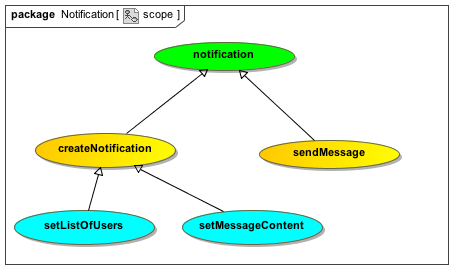
\includegraphics[width=0.5\textwidth]{Notification_Scope}}
	    	\caption{Notifications Scope}
	    	\label{fig:Notification_Scope}
   	\end{figure}
\subsubsection{Use cases}
\subsubsection{Domain model}
